\documentclass[a4paper, twocolumn, landscape, 9pt]{article}
\usepackage[utf8]{inputenc}
\usepackage[T1]{fontenc}
\usepackage{multicol}
\usepackage[margin=0.5in, bmargin=0.4in, tmargin=0.8in]{geometry}
\usepackage{titlesec}
\usepackage{etoolbox}
\usepackage{fancyhdr}
\usepackage[titles]{tocloft}
\usepackage{graphicx}
\usepackage{listings}
\usepackage{amsmath}
\usepackage{hyperref}
\usepackage{float}

\hypersetup{
  colorlinks,
  citecolor=black,
  filecolor=black,
  linkcolor=black,
  urlcolor=black
}

\pagestyle{fancy}
\fancyhf{}
\rhead{Page \thepage}
\lhead{Federal University of Bahia - Universidade Federal da Bahia}

\lstset{
language=R,
literate=
{≡}{{$\equiv$}}1
{∩}{{$\cap$}}1
{∪}{{$\cup$}}1
{∛N}{{$\sqrt[3]{N}$}}1
{Ã}{{\~A}}1
{Á}{{\'A}}1
{Â}{{\^A}}1
{á}{{\'a}}1
{à}{{\`a}}1
{ã}{{\~a}}1
{â}{{\^a}}1
{é}{{\'e}}1
{É}{{\'E}}1
{ê}{{\^e}}1
{í}{{\'i}}1
{ó}{{\'o}}1
{ô}{{\^o}}1
{õ}{{\~o}}1
{ú}{{\'u}}1
{ü}{{\"u}}1
{ç}{{\c{c}}}1
}

\usepackage{xcolor}
\usepackage{listings}
% \usepackage{courier}
\usepackage{courier}
\usepackage{pgfplotstable}
% recommended:
\usepackage{booktabs}
\usepackage{array}
\usepackage{colortbl}
\usepackage{verbatim}
\usepackage{xstring}

\definecolor{mygreen}{rgb}{0,0.6,0}
\definecolor{mygray}{rgb}{0.5,0.5,0.5}
\definecolor{mymauve}{rgb}{0.58,0,0.82}
\definecolor{codegreen}{rgb}{0,0.6,0}
\definecolor{codegray}{rgb}{0.5,0.5,0.5}
\definecolor{codepurple}{rgb}{0.58,0,0.82}
\definecolor{backcolour}{rgb}{0.95,0.95,0.92}

\def\trim#1{\ignorespaces#1\unskip} 

\lstset{ %
  basicstyle=\linespread{0.82}\footnotesize\ttfamily,        % the size of the fonts that are used for the code
  breakatwhitespace=true,         % sets if automatic breaks should only happen at whitespace
  breaklines=true,                 % sets automatic line breaking
  commentstyle=\itshape\color{black!63},    % comment style
  extendedchars=true,              % lets you use non-ASCII characters; for 8-bits encodings only, does not work with UTF-8
  frame=lbtr,                    % adds a frame around the code
  keepspaces=true,                 % keeps spaces in text, useful for keeping indentation of code (possibly needs columns=flexible)
  keywordstyle=\bfseries,       % keyword style
  numbers=left,                    % where to put the line-numbers; possible values are (none, left, right)
  numbersep=8pt,                   % how far the line-numbers are from the code
  numberstyle=\scriptsize, % the style that is used for the line-numbers
  rulecolor=\color{black},         % if not set, the frame-color may be changed on line-breaks within not-black text (e.g. comments (green here))
  showspaces=false,                % show spaces everywhere adding particular underscores; it overrides 'showstringspaces'
  showstringspaces=false,          % underline spaces within strings only
  showtabs=false,                  % show tabs within strings adding particular underscores
  stringstyle=,     % string literal style
  tabsize=2,                     % sets default tabsize to 2 spaces
  inputencoding=utf8
}

\lstdefinestyle{colored}{
  basicstyle=\footnotesize\ttfamily,
  keywordstyle=\color{green!30!black},
  commentstyle=\itshape\color{purple!40!black},
  identifierstyle=,
  stringstyle=\color{orange},
}

\lstdefinestyle{mystyle}{
  %backgroundcolor=\color{backcolour},   
  commentstyle=\color{green!30!black},
  keywordstyle=\color{magenta},
  numberstyle=\color{codegray},
  stringstyle=\color{codepurple},
  rulecolor=\color{codegray},
}

\lstset{columns=fullflexible}

\def\EOF{1000}

\def\normLineNumber#1{\trim{\detokenize{#1}}}

\newcommand{\includenote}[1]{\lstinputlisting{codes/#1}}
\newcommand{\includecode}[2][C++]{
  \lstinputlisting[escapechar=, language=#1]{codes/#2}
}

\newcommand{\includepiece}[3][C++]{
  %{\detokenize{#2} (\normLineNumber{#3})}
  \lstinputlisting[escapechar=, language=#1, linerange={#3}]{codes/#2}
}

% \pgfplotstabletypeset{col sep=tab}

\newcommand{\includetable}[1]{
  \begin{verbatim}\input{notes/#1}\end{verbatim}
}


% usage of commands
% section, subsection and subsubsection were renewed so they receive 2 arguments instead of 1. ex: \section{title}{text}
% \includecode[language]{file} include code from codes/{file}. default language is C++.
% \includepiece[language]{file}{firstline}{lastline} does the same thing, but it includes from firstline to lastline only.
%

%% Control the fonts and formatting used in the table of contents.

%% Aesthetic spacing redefines that look nicer to me than the defaults.

\setlength{\cftbeforesecskip}{0.02em}
\setlength{\cftbeforesubsecskip}{0.02em}
\setlength{\cftbeforesubsubsecskip}{0.02em}

%% Use Helvetica-Narrow Bold for Chapter entries

\renewcommand{\cftsecfont}{%
  \fontsize{10}{10}\usefont{T1}{phv}{bc}{n}\selectfont
}
\renewcommand{\cftsubsecfont}{
  \fontsize{9}{9}\usefont{T1}{phv}{c}{n}\selectfont
}
\renewcommand{\cftsubsubsecfont}{
  \fontsize{9}{9}\usefont{T1}{phv}{c}{n}\selectfont
}


\renewcommand{\familydefault}{\ttdefault}
\setlength{\columnsep}{1cm}

\let\Asection\section
\let\Bsection\subsection
\let\Csection\subsubsection

\renewcommand{\section}[2]{
  \ifstrequal{#2}{}{\Asection[#1 *]{#1} #2}{\Asection{#1} #2} %
}
\renewcommand{\subsection}[2]{
  \ifstrequal{#2}{}{\Bsection[#1 *]{#1} #2}{\Bsection{#1} #2} %
}
\renewcommand{\subsubsection}[2]{
  \ifstrequal{#2}{}{\Csection[#1 *]{#1} #2}{\Csection{#1} #2} %
}

\title{C++ Competitive Programming Library \\ \large ***DO NOT DISCLOSE OR DISTRIBUTE***}
\author{bfs.07 - Bernardo Flores Salmeron}
\date{}

\begin{document}

\titleformat{\section}[hang]{\large}{}{0pt}{\thesection. }
\titleformat{\subsection}[hang]{\normalsize}{}{0pt}{\thesubsection. }
\titleformat{\subsubsection}[hang]{\small}{}{0pt}{\thesubsubsection. }
\titlespacing{\section}{0px}{3px}{2px}
\titlespacing{\subsection}{0px}{2px}{1px}

% generate title and table of contents with no heading
\maketitle
\thispagestyle{fancy}

\makeatletter
%\renewcommand{\l@subsection}{\@dottedtocline{2}{1.5em}{3.0em}}
%\renewcommand{\l@subsubsection}{\@dottedtocline{3}{3.0em}{4em}}
\def\tableofcontents{\@starttoc{toc}}
\makeatother

%\centering\textcolor{red}{\textbf{THE WHOLE LIB USES dcmp() FOR FLOATING-POINT COMPARISON}}

\tableofcontents

\newpage

\section{Template}{
  \includecode{"template.cpp"}
}

\section{.Vscode}{

}

\section{Data Structures}{

  \subsection{Bit}{
    \includecode{"data_structures/bit.cpp"}
  }

  \subsection{Bit (Range Update)}{
    \includecode{"data_structures/bit_(range_update).cpp"}
  }

  \subsection{Bit 2D}{
    \includecode{"data_structures/bit_2d.cpp"}
  }

  \subsection{Merge Sort Tree}{
    \includecode{"data_structures/merge_sort_tree.cpp"}
  }

  \subsection{Min Queue}{
    \includecode{"data_structures/min_queue.cpp"}
  }

  \subsection{Mos Algorithm}{
    \includecode{"data_structures/mos_algorithm.cpp"}
  }

  \subsection{Ordered Set}{
    \includecode{"data_structures/ordered_set.cpp"}
  }

  \subsection{Persistent Segment Tree}{
    \includecode{"data_structures/persistent_segment_tree.cpp"}
  }

  \subsection{Segment Tree}{
    \includecode{"data_structures/segment_tree.cpp"}
  }

  \subsection{Segment Tree 2D}{
    \includecode{"data_structures/segment_tree_2d.cpp"}
  }

  \subsection{Segment Tree Beats}{
    \includecode{"data_structures/segment_tree_beats.cpp"}
  }

  \subsection{Segment Tree Polynomial}{
    \includecode{"data_structures/segment_tree_polynomial.cpp"}
  }

  \subsection{Sparse Table}{
    \includecode{"data_structures/sparse_table.cpp"}
  }

  \subsection{Sqrt Decomposition}{
    \includecode{"data_structures/sqrt_decomposition.cpp"}
  }

  \subsection{Treap}{
    \includecode{"data_structures/treap.cpp"}
  }

  \subsection{Treap Maximum Contigous Segment}{
    \includecode{"data_structures/treap_maximum_contigous_segment.cpp"}
  }

}

\section{Dp}{

  \subsection{Binary Lifting}{
    \includecode{"dp/binary_lifting.cpp"}
  }

  \subsection{Catalan}{
    \begin{figure}[H]
      \centering
      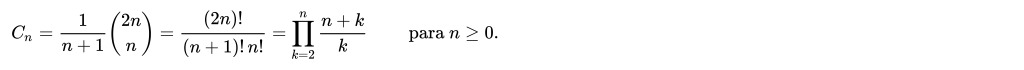
\includegraphics[scale=0.7]{"codes/dp/catalan.jpg"}
    \end{figure}
  }

  \subsection{Catalan 1 1 2 5 14 42 132}{
    \includecode{"dp/catalan_1_1_2_5_14_42_132.cpp"}
  }

  \subsection{Cht Optimization}{
    \includecode{"dp/cht_optimization.cpp"}
  }

  \subsection{Digit Dp}{
    \includecode{"dp/digit_dp.cpp"}
  }

  \subsection{Divide And Conquer Optimization}{
    \includecode{"dp/divide_and_conquer_optimization.cpp"}
  }

  \subsection{Edit Distance}{
    \includecode{"dp/edit_distance.cpp"}
  }

  \subsection{Knuth Optimization}{
    \includecode{"dp/knuth_optimization.cpp"}
  }

  \subsection{Lis}{
    \includecode{"dp/lis.cpp"}
  }

  \subsection{Longest Common Subsequence}{
    \includecode{"dp/longest_common_subsequence.cpp"}
  }

  \subsection{Longest Increasing Subsequence 2D (Not Sorted)}{
    \includecode{"dp/longest_increasing_subsequence_2d_(not_sorted).cpp"}
  }

  \subsection{Longest Increasing Subsequence 2D (Sorted)}{
    \includecode{"dp/longest_increasing_subsequence_2d_(sorted).cpp"}
  }

  \subsection{Subset Sum (Bitset)}{
    \includecode{"dp/subset_sum_(bitset).cpp"}
  }

}

\section{Graphs}{

  \subsection{All Eulerian Path Or Tour}{
    \includecode{"graphs/all_eulerian_path_or_tour.cpp"}
  }

  \subsection{Articulation Points}{
    \includecode{"graphs/articulation_points.cpp"}
  }

  \subsection{Bellman Ford}{
    \includecode{"graphs/bellman_ford.cpp"}
  }

  \subsection{Bipartite Check}{
    \includecode{"graphs/bipartite_check.cpp"}
  }

  \subsection{Block Cut Tree}{
    \includecode{"graphs/block_cut_tree.cpp"}
  }

  \subsection{Bridges}{
    \includecode{"graphs/bridges.cpp"}
  }

  \subsection{Centroid}{
    \includecode{"graphs/centroid.cpp"}
  }

  \subsection{Centroid Decomposition}{
    \includecode{"graphs/centroid_decomposition.cpp"}
  }

  \subsection{Compress Sccs In Dag}{
    \includecode{"graphs/compress_sccs_in_dag.cpp"}
  }

  \subsection{Count (3-4) Cycles}{
    \includecode{"graphs/count_(3-4)_cycles.cpp"}
  }

  \subsection{Cycle Detection}{
    \includecode{"graphs/cycle_detection.cpp"}
  }

  \subsection{De Bruijn Sequence}{
    \includecode{"graphs/de_bruijn_sequence.cpp"}
  }

  \subsection{Dijkstra + Dij Graph}{
    \includecode{"graphs/dijkstra_+_dij_graph.cpp"}
  }

  \subsection{Dinic}{
    \includecode{"graphs/dinic.cpp"}
  }

  \subsection{Dsu}{
    \includecode{"graphs/dsu.cpp"}
  }

  \subsection{Dsu On Tree}{
    \includecode{"graphs/dsu_on_tree.cpp"}
  }

  \subsection{Floyd Warshall}{
    \includecode{"graphs/floyd_warshall.cpp"}
  }

  \subsection{Functional Graph}{
    \includecode{"graphs/functional_graph.cpp"}
  }

  \subsection{Girth (Shortest Cycle In A Graph)}{
    \includecode{"graphs/girth_(shortest_cycle_in_a_graph).cpp"}
  }

  \subsection{Hld}{
    \includecode{"graphs/hld.cpp"}
  }

  \subsection{Hungarian}{
    \includecode{"graphs/hungarian.cpp"}
  }

  \subsection{Lca}{
    \includecode{"graphs/lca.cpp"}
  }

  \subsection{Longest Path In Dag}{
    \includecode{"graphs/longest_path_in_dag.cpp"}
  }

  \subsection{Maximum Independent Set (Set Of Vertices That Arent Directly Connected)}{
    \includecode{"graphs/maximum_independent_set_(set_of_vertices_that_arent_directly_connected).txt"}
  }

  \subsection{Maximum Path Unweighted Graph}{
    \includecode{"graphs/maximum_path_unweighted_graph.cpp"}
  }

  \subsection{Min Cost Flow Gpessoa}{
    \includecode{"graphs/min_cost_flow_gpessoa.cpp"}
  }

  \subsection{Min Cost Flow Katcl}{
    \includecode{"graphs/min_cost_flow_katcl.cpp"}
  }

  \subsection{Minimum Edge Cover (Set Of Edges That Are Adjacent To All Vertices)}{
    \includecode{"graphs/minimum_edge_cover_(set_of_edges_that_are_adjacent_to_all_vertices).txt"}
  }

  \subsection{Minimum Path Cover In Dag}{
    \begin{figure}[H]
      \centering
      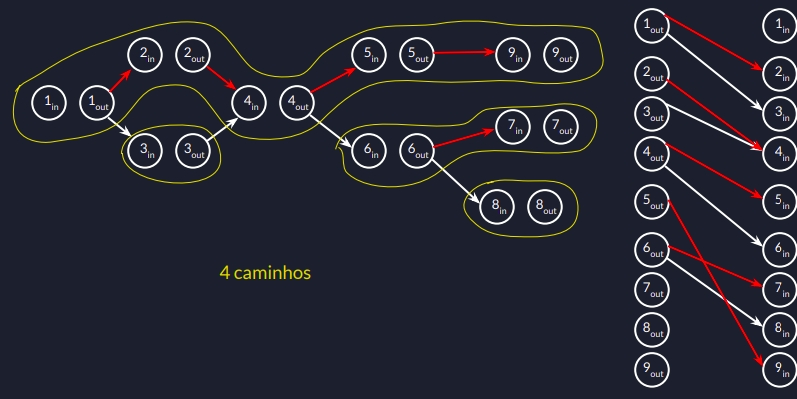
\includegraphics[scale=0.7]{"codes/graphs/minimum_path_cover_in_dag.jpg"}
    \end{figure}
  }

  \subsection{Minimum Path Cover In Dag}{
    \includecode{"graphs/minimum_path_cover_in_dag.txt"}
  }

  \subsection{Mst}{
    \includecode{"graphs/mst.cpp"}
  }

  \subsection{Number Of Different Spanning Trees In A Complete Graph}{
    \includecode{"graphs/number_of_different_spanning_trees_in_a_complete_graph.txt"}
  }

  \subsection{Number Of Ways To Make A Graph Connected}{
    \includecode{"graphs/number_of_ways_to_make_a_graph_connected.txt"}
  }

  \subsection{Pruffer Decode}{
    \includecode{"graphs/pruffer_decode.cpp"}
  }

  \subsection{Pruffer Encode}{
    \includecode{"graphs/pruffer_encode.cpp"}
  }

  \subsection{Pruffer Properties}{
    \includecode{"graphs/pruffer_properties.txt"}
  }

  \subsection{Remove All Bridges From Graph}{
    \includecode{"graphs/remove_all_bridges_from_graph.txt"}
  }

  \subsection{Scc (Kosaraju)}{
    \includecode{"graphs/scc_(kosaraju).cpp"}
  }

  \subsection{Small To Large (Merge Maps)}{
    \includecode{"graphs/small_to_large_(merge_maps).cpp"}
  }

  \subsection{Topological Sort}{
    \includecode{"graphs/topological_sort.cpp"}
  }

  \subsection{Tree Diameter}{
    \includecode{"graphs/tree_diameter.cpp"}
  }

  \subsection{Tree Distance}{
    \includecode{"graphs/tree_distance.cpp"}
  }

  \subsection{Tree Isomorphism}{
    \includecode{"graphs/tree_isomorphism.cpp"}
  }

}

\section{Language Stuff}{

  \subsection{Binary String To Int}{
    \includecode{"language_stuff/binary_string_to_int.txt"}
  }

  \subsection{Check Char Type}{
    \includecode{"language_stuff/check_char_type.cpp"}
  }

  \subsection{Check Overflow}{
    \includecode{"language_stuff/check_overflow.txt"}
  }

  \subsection{Counting Bits}{
    \includecode{"language_stuff/counting_bits.txt"}
  }

  \subsection{Gen Random Numbers (Rng)}{
    \includecode{"language_stuff/gen_random_numbers_(rng).cpp"}
  }

  \subsection{Int To Binary String}{
    \includecode{"language_stuff/int_to_binary_string.cpp"}
  }

  \subsection{Int To String}{
    \includecode{"language_stuff/int_to_string.cpp"}
  }

  \subsection{Permutation}{
    \includecode{"language_stuff/permutation.cpp"}
  }

  \subsection{Print Int128 T}{
    \includecode{"language_stuff/print_int128_t.cpp"}
  }

  \subsection{Read And Write From File}{
    \includecode{"language_stuff/read_and_write_from_file.cpp"}
  }

  \subsection{Readint}{
    \includecode{"language_stuff/readint.cpp"}
  }

  \subsection{Rotate Left}{
    \includecode{"language_stuff/rotate_left.cpp"}
  }

  \subsection{Rotate Right}{
    \includecode{"language_stuff/rotate_right.cpp"}
  }

  \subsection{Scanf From String}{
    \includecode{"language_stuff/scanf_from_string.cpp"}
  }

  \subsection{Split Function}{
    \includecode{"language_stuff/split_function.cpp"}
  }

  \subsection{String To Long Long}{
    \includecode{"language_stuff/string_to_long_long.cpp"}
  }

  \subsection{Substring}{
    \includecode{"language_stuff/substring.cpp"}
  }

  \subsection{Time Measure}{
    \includecode{"language_stuff/time_measure.cpp"}
  }

  \subsection{Unique Vector}{
    \includecode{"language_stuff/unique_vector.cpp"}
  }

  \subsection{Width}{
    \includecode{"language_stuff/width.cpp"}
  }

}

\section{Math}{

  \subsection{Bell Numbers}{
    \includecode{"math/bell_numbers.cpp"}
  }

  \subsection{Binary Exponentiation}{
    \includecode{"math/binary_exponentiation.cpp"}
  }

  \subsection{Chinese Remainder Theorem}{
    \includecode{"math/chinese_remainder_theorem.cpp"}
  }

  \subsection{Combinatorics}{
    \includecode{"math/combinatorics.cpp"}
  }

  \subsection{Diophantine Equation}{
    \includecode{"math/diophantine_equation.cpp"}
  }

  \subsection{Divide Fraction}{
    \includecode{"math/divide_fraction.cpp"}
  }

  \subsection{Divisors}{
    \includecode{"math/divisors.cpp"}
  }

  \subsection{Euler Totient}{
    \includecode{"math/euler_totient.cpp"}
  }

  \subsection{Extended Euclidean}{
    \includecode{"math/extended_euclidean.cpp"}
  }

  \subsection{Factorization}{
    \includecode{"math/factorization.cpp"}
  }

  \subsection{Fft}{
    \includecode{"math/fft.cpp"}
  }

  \subsection{Inclusion Exclusion}{
    \begin{figure}[H]
      \centering
      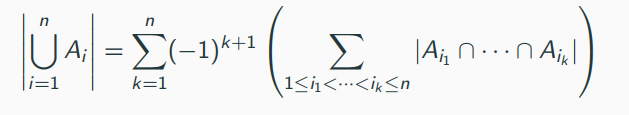
\includegraphics[scale=0.7]{"codes/math/inclusion_exclusion.jpg"}
    \end{figure}
  }

  \subsection{Inclusion Exclusion }{
    \includecode{"math/inclusion_exclusion_.cpp"}
  }

  \subsection{Karatsuba}{
    \includecode{"math/karatsuba.cpp"}
  }

  \subsection{Markov Chains}{
    \begin{figure}[H]
      \centering
      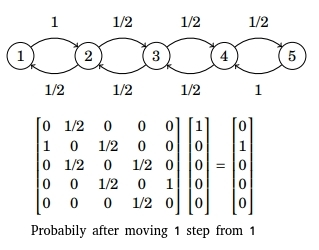
\includegraphics[scale=0.7]{"codes/math/markov_chains.jpg"}
    \end{figure}
  }

  \subsection{Matrix Exponentiation}{
    \begin{figure}[H]
      \centering
      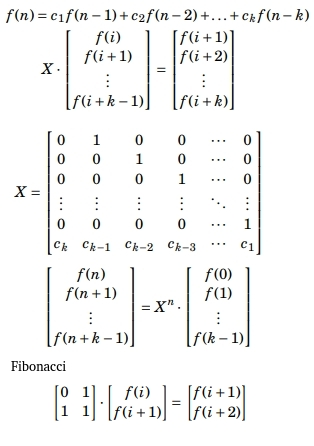
\includegraphics[scale=0.7]{"codes/math/matrix_exponentiation.jpg"}
    \end{figure}
  }

  \subsection{Matrix Exponentiation }{
    \includecode{"math/matrix_exponentiation_.cpp"}
  }

  \subsection{Pollard Rho (Factorize)}{
    \includecode{"math/pollard_rho_(factorize).cpp"}
  }

  \subsection{Pollard Rho (Find A Divisor)}{
    \includecode{"math/pollard_rho_(find_a_divisor).cpp"}
  }

  \subsection{Polynomial Convolution}{
    \includecode{"math/polynomial_convolution.cpp"}
  }

  \subsection{Primality Check}{
    \includecode{"math/primality_check.cpp"}
  }

  \subsection{Primes}{
    \includecode{"math/primes.txt"}
  }

  \subsection{Sieve + Segmented Sieve}{
    \includecode{"math/sieve_+_segmented_sieve.cpp"}
  }

  \subsection{Stars And Bars}{
    \begin{figure}[H]
      \centering
      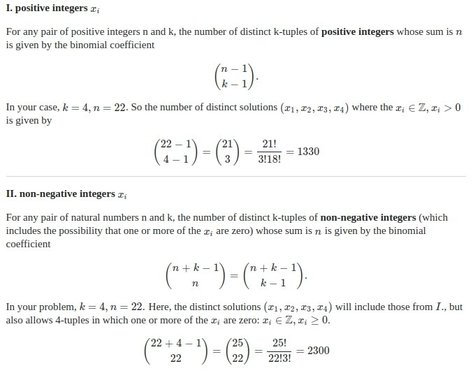
\includegraphics[scale=0.7]{"codes/math/stars_and_bars.jpeg"}
    \end{figure}
  }

}

\section{Miscellaneous}{

  \subsection{Counting Frequency Of Digits From 1 To K}{
    \includecode{"miscellaneous/counting_frequency_of_digits_from_1_to_k.py"}
  }

  \subsection{Counting Number Of Digits Up To N}{
    \includecode{"miscellaneous/counting_number_of_digits_up_to_n.cpp"}
  }

  \subsection{Infix To Postfix}{
    \includecode{"miscellaneous/infix_to_postfix.cpp"}
  }

  \subsection{Interval Scheduling}{
    \begin{figure}[H]
      \centering
      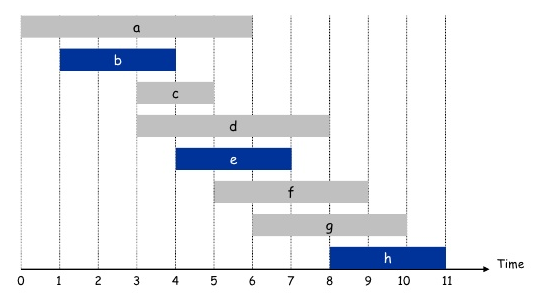
\includegraphics[scale=0.7]{"codes/miscellaneous/interval_scheduling.jpg"}
    \end{figure}
  }

  \subsection{Interval Scheduling}{
    \includecode{"miscellaneous/interval_scheduling.txt"}
  }

  \subsection{Iterate Over Subsets Of Mask}{
    \includecode{"miscellaneous/iterate_over_subsets_of_mask.cpp"}
  }

  \subsection{Kadane}{
    \includecode{"miscellaneous/kadane.cpp"}
  }

  \subsection{Kadane (Segment Tree)}{
    \includecode{"miscellaneous/kadane_(segment_tree).cpp"}
  }

  \subsection{Kadane 2D}{
    \includecode{"miscellaneous/kadane_2d.cpp"}
  }

  \subsection{Largest Area In Histogram}{
    \includecode{"miscellaneous/largest_area_in_histogram.cpp"}
  }

  \subsection{Point Compression}{
    \includecode{"miscellaneous/point_compression.cpp"}
  }

  \subsection{Ternary Search}{
    \includecode{"miscellaneous/ternary_search.cpp"}
  }

  \subsection{Tower Of Hanoi}{
    \includecode{"miscellaneous/tower_of_hanoi.cpp"}
  }

  \subsection{Two Sat}{
    \includecode{"miscellaneous/two_sat.cpp"}
  }

}

\section{Stress Testing}{

  \subsection{Check}{
    \includecode{"stress_testing/check.sh"}
  }

  \subsection{Gen}{
    \includecode{"stress_testing/gen.cpp"}
  }

  \subsection{Run}{
    \includecode{"stress_testing/run.sh"}
  }

}

\section{Strings}{

  \subsection{Aho Corasick}{
    \includecode{"strings/aho_corasick.cpp"}
  }

  \subsection{Hashing}{
    \includecode{"strings/hashing.cpp"}
  }

  \subsection{Kmp}{
    \includecode{"strings/kmp.cpp"}
  }

  \subsection{Lcs K Strings}{
    \includecode{"strings/lcs_k_strings.cpp"}
  }

  \subsection{Lexicographically Smallest Rotation}{
    \includecode{"strings/lexicographically_smallest_rotation.cpp"}
  }

  \subsection{Manacher (Longest Palindrome)}{
    \includecode{"strings/manacher_(longest_palindrome).cpp"}
  }

  \subsection{Suffix Array}{
    \includecode{"strings/suffix_array.cpp"}
  }

  \subsection{Suffix Array Mine}{
    \includecode{"strings/suffix_array_mine.cpp"}
  }

  \subsection{Suffix Automaton}{
    \includecode{"strings/suffix_automaton.cpp"}
  }

  \subsection{Trie}{
    \includecode{"strings/trie.cpp"}
  }

  \subsection{Z Function}{
    \includecode{"strings/z_function.cpp"}
  }

}

\end{document}
